\documentclass[a4paper,12pt,obeyspaces,spaces,hyphens]{article}

\usepackage{agenda}
\usepackage{colortbl}
\usepackage{xcolor}
\usepackage{palatino}
\usepackage{calc}

\hypersetup{pdftitle={Embedded Linux system development},
  pdfauthor={\vendor}}

\begin{document}

\thispagestyle{fancy}

\setlength{\arrayrulewidth}{0.8pt}

\begin{center}
\LARGE
Embedded Linux system development\\
\large
5-day session
\end{center}
\vspace{1cm}

\small
\newcolumntype{g}{>{\columncolor{darkagendacolor}}m{4cm}}
\newcolumntype{h}{>{\columncolor{lightagendacolor}}X}

\arrayrulecolor{lightgray} {
  \setlist[1]{itemsep=-5pt}
  \begin{tabularx}{\textwidth}{|g|h|}
    {\bf Title} & Embedded Linux system development \\
    \hline

    {\bf Overview} &
    Introduction to Embedded Linux \par
    Cross-Compiling Toolchains \par
    Bootloaders \par
    Linux Kernel Introduction \par
    Linux Root Filesystems \par
    Embedded Linux System Development \par
    Embedded Linux Application Development \par
    Real Time in Embedded Linux Systems \par
    Practical labs with the ARM-based Beagle Bone Black.\\
    \hline

    {\bf Duration} & {\bf Five} days - 40 hours (8 hours per day).
    \newline 50\% of lectures, 50\% of practical labs. \\
    \hline

    {\bf Trainer} & \kerneltrainers
    \newline \trainingurl\\
    \hline

    {\bf Language} & Oral lectures: English, \locallanguage.
    \newline Materials: English.\\
    \hline

    {\bf Audience} & People developing devices using Linux
    \newline People supporting embedded Linux system developers. \\
    \hline

    {\bf Prerequisites} &

    {\bf Solid experience in C programming}
    \newline In particular, participants must be familiar
    with creating and dealing with complex data types and structures,
    with pointers to such symbols, as well as with function pointers.
    \newline {\bf Knowledge and practice of UNIX or GNU/Linux commands}
    \newline People lacking experience on this topic should get
    trained by themselves with our freely available on-line slides
    (\url{http://free-electrons.com/docs/command-line/}).
    \\
    \hline
  \end{tabularx}

  \begin{tabularx}{\textwidth}{|g|h|}
    {\bf Required equipment} &
    {\bf For on-site sessions only}
    \newline Everything is supplied by \vendor \hspace{1 mm}
    in public sessions.
    \begin{itemize}
    \item Video projector 
    \item PC computers with at least 4 GB of RAM, and {\bf Ubuntu Linux 12.04 (x64)}
    installed in a {\bf free partition of at least 60 GB}. We don't support other
    distributions, because we can't test all possible package versions.
    {\bf Using Linux in a virtual machine is not supported}, because of issues
    connecting to real hardware.

    \item Labs should be run on \hostmachine or better.
    \item {\bf Connection to the Internet} (direct or through the
    company proxy).
    \item {\bf PC computers with valuable data must be backed up}
    before being used in our sessions.  Some people have already made
    mistakes during our sessions and damaged work data.
    \item It is a good idea to do a fresh install on a new disk
      which subsuquently can be used as an external USB disk.
    \end{itemize} \\
    \hline

    {\bf Materials} & Print and electronic copies of presentations and
    labs.
    \newline Electronic copy of lab files.\\
    \hline

    {\bf Credits} & This material is developed by Free-Electrons \localauthor .\\
    \hline

\end{tabularx}}

\normalsize
\clearpage

\feagendatwocolumn
{Hardware}
{
  The hardware platform used for the practical labs of this training
  session is the {\bf BeagleBone Black}, which features:

  \begin{itemize}
  \item An ARM AM335x processor from Texas Instruments (Cortex-A8
    based), 3D acceleration, etc.
  \item 512 MB of RAM
  \item 2 GB of on-board eMMC storage
  \item USB host and device
  \item HDMI output
  \item 2 x 46 pins headers, to access UARTs, SPI busses, I2C busses
    and more.
  \end{itemize}
}
{}
{
  \begin{center}
    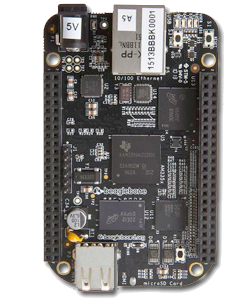
\includegraphics[height=5cm]{agenda/beagleboneblack.png}
  \end{center}
}

\feagendaonecolumn
{Labs}
{
  The practical labs of this training session use the following
  hardware peripherals to illustrate the development of Linux device
  drivers:

  \begin{itemize}
  \item A high-speed micro-SD card (minimum 4 GB)
  \item A SD-Card Reader
  \item USB - Ethernet adapter.
      The Ethernet will be reconfigured, and if you do not 
      want to change your normal setup, an USB - Ethernet adapter is OK.
  \item USB - Serial Adapter
  \item Two free USB ports for USB, or an external powered USB hub.
  \end{itemize}
}

\clearpage
\section{Day 1 - Morning}

\feagendatwocolumn
{Lecture - Introduction to Embedded Linux}
{
  \begin{itemize}
  \item Advantages of Linux and open source for embedded systems
  \item A few examples of embedded systems running linux
  \item Embedded Hardware for Linux systems
  \item Embedded Linux system architecture
  \end{itemize}
}
{Lab - Training Setup}
{
  \begin{itemize}
  \item Install the Lab archives
 \end{itemize}
}
\section{Day 1 - Afternoon}
\feagendatwocolumn
{Lecture - Cross Compiling Toolchains}
{
  \begin{itemize}
  \item Definitions and Components
  \item C Libraries
  \item Toolchain Options
  \item Obtaining a Toolchain
  \end{itemize}
}
{Lab - Cross Compiling a toolchain}
{
  \begin{itemize}
  \item Building a Yocto SDK
  \item Configuring Crosstool-NG
  \item Build a toolchain
  \item Getting a free commercially supported toolchain (Sourcery)
 \end{itemize}
}
\clearpage
\section{Day 2 - Morning}
\feagendatwocolumn
{Lecture - Bootloaders}
{
  \begin{itemize}
  \item Boot Sequence
  \item The U-Boot Bootloader
  \end{itemize}
}
{Lab - U-Boot}
{
  {\em Using the BeagleBoneBlack}
  \begin{itemize}
  \item Communication with the board using a serial console
  \item Configure, Build and Install U-Boot
  \item Learn U-Boot commands
  \item Setup TFTP communications
  \end{itemize}
}

\section{Day 2 - Afternoon}
\feagendatwocolumn
{Lecture - Linux kernel Introduction}
{
  \begin{itemize}
  \item Linux Features
  \item Linux Versioning Schemes
  \item Linux Kernel Sources
  \item Kernel Configuration
  \item Compiling and Installing the Kernel for the host
  \item Cross-Compilining the kernel
  \item Using kernel modules
  \end{itemize}
}
{Lab - Kernel cross-compiling}
{
  {\em Using the BeagleBoneBlack}
  \begin{itemize}
  \item Set up the cross compiling environment
  \item Configure the kernel using Kconfig
  \item Cross-compile for an ARM platform
  \item Boot the kernel
  \end{itemize}
}

\clearpage
\section{Day 3 - Morning}

\feagendatwocolumn
{Lecture - Linux Root Filesystem}
{
  \begin{itemize}
  \item Principle and solutions
  \item Contents
  \item Device Files
  \item Virtual File Systems
  \item Minimal File Systems
  \item Busybox
  \end{itemize}
}
{Lab - A tiny embedded systems} 
{
  \begin{itemize}
  \item Make linux boot using NFS
  \item Configure and Create a minuimalistic Linux embedded system
  \item Install and use Busybox
  \item System startup with /sbin/init
  \item Setup a simple web interface
  \item Use shared libraries
  \end{itemize}
}

\section{Day 3 - Afternoon}

\feagendatwocolumn
{Lecture - Block Filesystems}
{
  \begin{itemize}
  \item Difference vs Flash file systems
  \item Devices
  \item Traditional file systems (ext2,vfat)
  \item Journalled file systems (ext3,ext4)
  \item Filesystem recovery
  \item Mounting filesystems
  \item Squashfs
  \item Tmpfs
  \end{itemize}
}
{Lab - Block Filesystems}
{
  {\em Using the BeagleBoneBlack}
  \begin{itemize}
  \item Creating partitions
  \item Booting with a mix of filesystems
  \end{itemize}
}
\\
\feagendatwocolumn
{Lecture - Flash Filesystems}
{
  \begin{itemize}
  \item The MTD subsystem
  \item MTD partitions
  \item JFFS2
  \item Yaffs
  \item UBI
  \end{itemize}
}
{Lab - Block Filesystems}
{
  {\em Using the BeagleBoneBlack}
  \begin{itemize}
  \item Note: this lab needs revising, Beaglebone does not have NAND Flash
  \item Note: Needs to show UBI
  \item Creating partitions on flash storage
  \item Read-Only JFFS2
  \item Read-Write JFFS2
  \end{itemize}
}

\clearpage
\section{Day 4 - Morning}

\feagendatwocolumn
{Lecture - Embedded Linux system development}
{
  \begin{itemize}
  \item Open Source components and licensing
  \item Networking
  \item System Utilities
  \item Language Interpreters
  \item Audio, Video and Multimedia
  \item Graphical Toolkits
  \item Databases
  \item Web Browsers
  \item Examples
  \end{itemize}
}
{Lab - Manual cross-compiling}
{
  {\em Using the BeagleBoneBlack}
  \begin{itemize}
  \item Manual cross-compiling applications and libraries
  \item Common techniques and issues
  \end{itemize}
}
\\
\section{Day 4 - Afternoon}
\feagendatwocolumn
{Lecture - Build Systems}
{
  \begin{itemize}
  \item System Building
  \item Commercial Linux solutions
  \end{itemize}
}
{Lab - Buildroot}
{
  {\em Using the BeagleBoneBlack}
  \begin{itemize}
  \item Rebuilding using Buildroot
  \item Adding your own DirectFB based application
  \end{itemize}
}

\clearpage
\section{Day 5 - Morning}
\feagendatwocolumn
{Lecture - Embedded Linux application development}
{
  \begin{itemize}
  \item Developing applications on embedded linux
  \item Integrated development environment
  \item Version Control Systems
  \item Debuggers
  \item Remote debugging
  \item Memory checkers
  \item System analysis
  \item (Not) Developing on Windows
  \end{itemize}
}
{Lab - Application Development and debugging}
{
  {\em Using the BeagleBoneBlack}
  \begin{itemize}
  \item Compile your own application
  \item Set up remote debugging
  \item Debug a simple application
  \end{itemize}
}

\section{Day 5 - Afternoon}
\feagendatwocolumn
{Lecture - Real-time in embedded linux systems}
{
  \begin{itemize}
  \item PREEMPT\_RT
  \item Real time extensions
  \item Xenomai
  \end{itemize}
}
{Lab - Real-time}
{
  {\em Using the BeagleBoneBlack}
  \begin{itemize}
  \item Check Clock accuracy
  \item Build a POSIX real-time application 
  \item Build a Xenomai real-time application
  \item Compare the two solutions
  \end{itemize}
}
\end{document}

